\begin{Introducao} % ---------------------------------------------------------------
\secaoprimaria{Introdução}
% ============================================================================
% INTRODUÇÃO - EDITE O TEXTO ABAIXO
% ============================================================================
A FAI - Centro de Ensino Superior em Gestão, Tecnologia e Educação (FAI), por meio da sua biblioteca, disponibiliza este manual para normalização de trabalhos acadêmicos para os seus alunos, professores e funcionários. Este material é essencial ao uso das normas técnicas para uma apresentação correta e melhor compreensão da leitura, uma vez que um trabalho de nível superior, ou de pós-graduação, é analisado por uma banca examinadora composta por profissionais diversos, de elevado nível de conhecimentos sobre o assunto.

A normalização adotada neste manual tem como base, as normas de documentação da Associação Brasileira de Normas Técnicas (ABNT), tais como:
\begin{alinea}
    \item BNT NBR 6023:2002 - Informação e documentação - Referências - Elaboração;
    \item ABNT NBR 6024:2012 - Informação e documentação - Numeração Progressiva das seções de um documento escrito - apresentação;
    \item ABNT NBR 6027:2012 - Informação e documentação - Sumário - apresentação;
    \item ABNT NBR 6028:2003 - Informação e documentação;
    \item ABNT NBR 6034:2004 - Informação e documentação - Índice – apresentação;
    \item ABNT NBR 10520:2002 - Informação e documentação - Citação em documentos - apresentação;
    \item ABNT NBR 12225:2004 - Informação e documentação - Lombada – apresentação;
    \item ABNT NBR 14724:2011 - Informação e documentação - Trabalhos Acadêmicos - apresentação.
\end{alinea}

Devido à atualização dos padrões nacionais e internacionais, fez-se necessária mais uma revisão no manual, que por sua vez, encontra-se em sua 8ª edição. A apresentação gráfica dos textos científicos é regulamentada pela ABNT, pois segue o padrão básico internacional, o qual organiza e permite a identificação de formas e origens de textos científicos em todo o mundo (SANTOS, 2001). É importante ressaltar que em alguns casos a ABNT apresenta em suas normas algumas regras que são opcionais, permitindo que a instituição defina seus próprios critérios. Por isso, a FAI decidiu pela utilização de alguns critérios mencionados neste manual para promover a padronização e facilitar a compreensão da comunidade acadêmica acerca da realização de seus trabalhos acadêmico/científicos.
% FIM: INTRODUÇÃO ============================================================
\end{Introducao}





\begin{Desenvolvimento} % ------------------------------------------------------------------
% ============================================================================
% DESENVOLVIMENTO- EDITE O TEXTO ABAIXO. É O CONTEÚDO PRINCIPAL DO TRABALHO
% ============================================================================

\secaoprimaria{Trabalhos Acadêmicos}
A NBR 14724 (ABNT, 2011) especifica os princípios gerais para a elaboração de trabalhos acadêmicos (teses, dissertações, trabalhos de conclusão de curso, monografias e outros trabalhos similares), visando sua apresentação à Instituição de Ensino, a bancas e comissões examinadoras compostas por professores, especialistas, designados e/ou outros.

\secaosecundaria{Definições}
Seguem as definições da NBR 14724 (ABNT, 2011) e da NBR 6022 (ABNT, 2003), para trabalhos acadêmicos e artigos:

\begin{alinea}
    \item Dissertação: documento que apresenta o resultado de um trabalho experimental ou exposição de um estudo científico retrospectivo, de tema único e bem delimitado em sua extensão, com o objetivo de reunir, analisar e interpretar informações. Deve evidenciar o conhecimento da literatura existente sobre o assunto e a capacidade de sistematização do candidato. É feito sob a coordenação de um orientador (Doutor), visando à obtenção do título de mestre.
    \item Tese: documento que representa o resultado de um trabalho experimental ou exposição de um estudo científico de tema único e bem delimitado. Deve ser elaborado com base em investigação original, constituindo-se em real contribuição para a especialidade em questão. É feito sob a coordenação de um orientador (Doutor) e visa a obtenção do título de doutor, ou similar.
    \item Trabalho de conclusão de graduação, trabalho de graduação interdisciplinar, trabalho de conclusão de curso de especialização e/ou aperfeiçoamento: documento que apresenta o resultado de estudo, devendo expressar conhecimento do assunto escolhido, que deve ser obrigatoriamente emanado da disciplina, módulo, estudo independente, curso, programa ou outros ministrados. Deve ser feito sob a coordenação de um Professor orientador.
    \item Artigo científico: parte de uma publicação com autoria declarada, que apresenta e discute ideias, métodos, técnicas, processos e resultados nas diversas áreas do conhecimento.
\end{alinea}

Santos (2001, p. 37) conceitua monografia como:
\begin{citacaodireta}
Um texto de primeira mão resultante de pesquisa científica e que contém a identificação, o posicionamento, o tratamento, e o fechamento competente de um tema/problema que essencialmente analisa, em que o objeto (o tema, o problema é geralmente bem delimitado em extensão, a monografia permite o aprofundamento do estudo). Fundamenta-se na organização e na interpretação analítica e avaliativa de dados, conforme objetivos (linhas de raciocínio) pré-estabelecidos. A matéria prima do raciocínio são os dados, que basicamente se constituem de axiomas científicos (verdadeiros aceitos por diversas ciências), da autoridade de autores consagrados, com suas ilustrações, testemunhos e, até mesmo, da sua experiência pessoal coerente de pesquisador. O raciocínio é desenvolvido de forma indutiva (parte-se de experiências e observações particulares para se chegar a um princípio geral), ou de forma dedutiva (parte-se de um principio geral para verificá-la em casos particulares).
\end{citacaodireta}

Segundo França e Vasconcelos (2008) a monografia, por ser uma primeira experiência de relato científico, constitui-se numa preparação metodologia para futuras investigações. Conforme Salomon (1979, p. 36),

\begin{citacaodireta}
O trabalho científico é identificado, frequentemente, com a investigação científica ou com o seu resultado, quando este é comunicado. Perfeitamente válida a identificação, uma vez que dá à investigação o seu devido lugar e, ao mesmo tempo, mostra a importância da comunicação no processo de elaboração dos trabalhos científicos.
\end{citacaodireta}

Definidos, de forma bastante resumida, os vários tipos de trabalhos científicos existentes, passa- se às informações sobre a estrutura de composição desses documentos.

\secaosecundaria{Estrutura}
A estrutura de trabalhos acadêmicos (ou científicos) tais como relatórios de estágio, artigos e monografias, compreende os seguintes elementos: parte externa, pré-textuais, textuais e pós- textuais, conforme mostra a Figura: \ref{figura:EstruturaTrabalhoAcademico}.

\begin{figura}[h!]
  \centering
  \addfigura
  \includegraphics[width=1\textwidth]{ilustracoes/figuras/Estrutura de trabalho acadêmico.png}
  \legenda{Estrutura de trabalhos acadêmicos, monografias e relatórios de estágio}
  \fonte{O autor}
  \label{figura:EstruturaTrabalhoAcademico}
\end{figura}

O Quadro \ref{quadro:EspecificacaoElementos} especifica os elementos em função do tipo de trabalho. Note-se que nas partes pré- textuais e pós-textuais há elementos de inclusão obrigatória, opcional e condicional (opcional, mas com indicação de inclusão em determinados casos). Já as partes textuais são obrigatórias para todos os tipos de documentos acadêmico-científicos.

\begin{quadro} [h!]
  \centering
  \addquadro
  \includegraphics[width=1\textwidth]{ilustracoes/quadros/Especificação de Elementos.png}
  \legenda{Especificação de elementos em função do tipo de trabalho}
  \fonte{Equipe do Núcleo de Pós-Graduação da FAI}
  \label{quadro:EspecificacaoElementos}
\end{quadro}

\secaoprimaria{Regras gerais de apresentação}
Os trabalhos acadêmicos devem ser apresentados formalmente conforme as especificações descritas nas seções a seguir. Ver síntese no Apêndice A.

\secaosecundaria{Formato}
Os textos devem ser apresentados em papel branco, formato A4 (21cm x 29,7cm) digitados na cor preta, com exceção das ilustrações, que podem ser coloridas. O documento deve ser produzido usando-se apenas um lado do papel. Livros e periódicos cujos formatos são definidos pela editora constituem exceções a essa regra, conforme NBR 14724 (ABNT, 2011).

As folhas devem apresentar margens superior e esquerda de 3 cm e inferior e direita de 2 cm. Recomenda-se, para digitação, utilizar a fonte Times New Roman, tamanho 12 para o texto e tamanho menor (opta-se por tamanho 10) para citações de mais de três linhas, notas de rodapé, paginação e legendas das ilustrações e tabelas. Utiliza-se o estilo itálico para nomes científicos e expressões estrangeiras, caso ocorram no texto.

Todas as folhas, incluindo-se a capa, folha de rosto, folha de aprovação, dedicatória, agradecimentos, epígrafe, resumo, abstract, listas, sumário, são contadas e numeradas com romanos minúsculos, ou não numeradas. Os números de páginas não são visualizados na capa, nem na primeira página de cada capítulo, conforme NBR 14724 (ABNT, 2011).

Existe um modelo-padrão segundo as NBR 6024 (ABNT, 2012) e NBR 14724 (ABNT, 2011) para se colocar a numeração das páginas: a visualização do número da página, em algarismos arábicos, começa a partir da segunda folha da parte textual (Introdução) no canto superior direito da folha, usando fonte Times New Roman número 10.

Os elementos textuais (Introdução, Desenvolvimento e Conclusão) e pós-textuais (referências, obras consultadas, glossário, apêndice e anexo) são contados e numerados (isto é, a numeração da página é visualizada). Quando o trabalho for composto por 2 (dois) ou mais volumes, mantém-se uma única sequência de numeração das folhas, do primeiro ao último volume. As folhas dos apêndices e anexos devem ser numeradas de maneira contínua e sua paginação dá seguimento à do texto principal.

Obs.: Trabalhos de monografias devem ter um mínimo de trinta (30) e um máximo de sessenta (60) páginas, incluindo anexos; e os artigos um máximo de 20 páginas.

Todo o texto é digitado com espaçamento 1,5 entre linhas, com 12 pontos antes e 12 pontos depois de cada parágrafo, excetuando-se as citações de mais de três linhas, notas de rodapé, legendas das ilustrações, tabelas e referências, a natureza do trabalho, o objetivo, o nome da Instituição a que é submetida e a área de concentração (que se apresentam na folha de rosto), que devem ser digitados em espaço simples. As referências, ao final do trabalho, devem utilizar entrelinhas simples separadas entre si por uma linha em branco.

Quanto à separação entre títulos, subtítulos e texto, observa-se o seguinte:

\begin{alinea}
  \item os títulos de capítulos estão sempre no início de uma nova página; não há texto antes deles, portanto;
  \item separação entre títulos e subtítulos de capítulos e texto: entre linhas de 1,5 com espaçamento de 12 pontos antes e depois, exatamente como a separação de parágrafos;
  \item formatação do texto, incluindo-se títulos e subtítulos: entre linhas de 1,5 com 12 pontos antes e 12 pontos depois;
  \item separação entre o texto e os subtítulos: pula-se uma linha em branco.
\end{alinea}

Conforme NBR 10520 (ABNT, 2002), para a paragrafação de um trabalho científico podem ser utilizados dois estilos: o parágrafo sem recuo ou com recuo da margem. No caso de se optar pelo parágrafo com recuo, a primeira linha do parágrafo terá recuo de 1,25 cm da margem esquerda. No caso de se optar pelo parágrafo sem recuo, o modelo adotado pela FAI, ele deve ser justificado, separando-se os parágrafos com 12 pontos antes e 12 pontos depois, exatamente como o texto já se encontra formatado. Qualquer que seja a modalidade escolhida, deve-se utilizar o mesmo estilo de paragrafação no documento inteiro.

As formas abreviadas de nomes abreviaturas e siglas são usadas para evitar a repetição de palavras e expressões frequentemente utilizadas no texto (FRANÇA; VASCONCELOS, 2008). Quando for usar sigla no texto do trabalho, deve-se observar o seguinte: a primeira vez que a sigla aparecer no texto, ela deve vir precedida pelo nome completo por extenso e, em seguida, deve-se colocá-la entre parênteses;

\listaalinhada{Exemplo}{
  Associação Brasileira de Normas Técnicas (ABNT) \\
  Instituto Brasileiro de Geografia e Estatística (IBGE) \\
  Fundação Vale do Taquari de Educação e Desenvolvimento Social (FUVATES)
}

Quando a obra tiver mais de um volume, todos os volumes deverão apresentar folha de rosto, destacando-se a indicação "Volume I" e "Volume II" logo abaixo do título ou subtítulo, se houver. A numeração das folhas dos outros volumes deve ser uma sequência natural do primeiro volume.

\secaosecundaria{Equações e Fórmulas}
Quando houver equações e fórmulas no texto, elas devem aparecer destacadas, de modo a facilitar a sua leitura. Na sequência normal do texto é permitido o uso de uma entrelinha maior que comporte seus elementos (expoentes, índice e outros).

Quando as equações e fórmulas vierem destacadas do parágrafo são centralizadas e, se necessário, deve-se numerá-las. Caso venham fragmentadas em mais de uma linha, por falta de espaço, devem ser interrompidas antes do sinal de igualdade ou depois dos sinais de adição, subtração, multiplicação, ou divisão.

Exemplo: As chamadas equações e fórmulas no texto devem ser feitas da seguinte forma:

\begin{equacao}
x^2 + y^2 = z^2 \label{eq:pythagoras}
\end{equacao}
\begin{equacao}
(x^2 + y^2) = n \label{eq:pythagoras2}
\end{equacao}
\begin{equacao}
x = \frac{-b \pm \sqrt{b^2-4ac}}{2a}
\end{equacao}
\begin{equacao}
(1 + x)^n = 1 + \frac{nx}{1!} + \frac{n(n-1)x^2}{2!} + \cdots
\end{equacao}

\secaoprimaria{Divisão do trabalho}
Adota-se a numeração progressiva, seguindo a norma NBR 6024 (ABNT, 2012) para se fazer as divisões e subdivisões do texto, evidenciando-se, assim, a sistematização do conteúdo do trabalho. Em um trabalho acadêmico, as principais divisões são nomeadas como seções primárias, as quais podem ser subdivididas em seções secundárias, que por sua vez podem ser ainda divididas em seções terciárias e assim por diante. Ultrapassar a quarta seção não é recomendável.

As seções primárias, por serem as principais divisões de um texto, devem iniciar-se em folha distinta. Devem-se empregar algarismos arábicos em um número ou grupo de números antes do título das seções ou subseções, permitindo-se, assim, sua localização imediata. As seções primárias são indicadas pela sequência dos números inteiros a partir do número um. Já a indicação de seção secundária é constituída pelo número indicativo da seção primária a que pertence, seguida do número que lhe será atribuído à sequência e separada por ponto. O mesmo processo deverá ser repetido para as demais seções.

Formatação a ser seguida:

\begin{alinea}
  \item seções primárias: os títulos dessas seções devem ser em caixa alta, fonte 12 e em negrito;
  \item seções secundárias: os títulos dessas seções devem ser iguais aos das primárias, porém sem negrito;
  \item seções terciárias: os títulos dessas seções devem ser em negrito, somente com a primeira letra maiúscula;
  \item seções quaternárias: iguais às terciárias, porém sem negrito;
  \item seções quinárias (se forem absolutamente necessárias): iguais às quaternárias.
\end{alinea}

Modelo:
2 SEÇÃO PRIMÁRIA
2.1 SEÇÃO SECUNDÁRIA
2.1.1 Seção terciária
2.1.1.1 Seção quaternária
2.1.1.1.1 Seção quinária

Exemplo, segundo Rodrigues (2007):
3 USABILIDADE X DESIGN DAS APLICAÇÕES
3.1 IMAGENS E LAYOUT
3.2 PROJETANDO A USABILIDADE
3.3 PROJETO DE INTERFACE COM O USUÁRIO
3.4 DESIGN CENTRADO NO USUÁRIO
3.4.1 Análise e modelagem de usuários

\secaosecundaria{Alíneas}
De acordo com a NBR 6024 (ABNT, 2012), a alínea é cada uma das subdivisões de um documento. Quando for necessário enumerar os diversos assuntos de uma seção que não possua título, esta deve ser subdividida em alíneas. A disposição gráfica das alíneas obedece às seguintes regras:

\begin{alinea}
  \item os diversos assuntos que não possuem título próprio, dentro de uma mesma seção, devem ser subdivididos em alíneas;
  \item o texto que antecede as alíneas termina em dois pontos;
  \item as alíneas devem ser indicadas alfabeticamente, em letra minúscula, seguida de parêntese fechado. Utilizam-se letras dobradas, quando esgotadas as letras do alfabeto;
  \item as letras indicativas das alíneas devem apresentar recuo de 0,5 cm em relação à margem esquerda;
  \item o texto da alínea deve começar por letra minúscula e terminar em ponto-e-vírgula, exceto a última alínea que termina em ponto final;
  \item o texto da alínea deve terminar em dois pontos, se houver subalínea;
  \item a segunda e as seguintes linhas do texto da alínea começam sob a primeira letra do texto da própria alínea;
  \item Entre as alíneas, inclusive a primeira delas, os parágrafos são formatados com zero ponto ante e zero depois;
  \item O próximo parágrafo, após a última alínea, volta a ter formatação normal com 12 pontos antes e 12 depois.
\end{alinea}

\secaoprimaria{Estrutura}
A estrutura de trabalhos acadêmicos compreende: elementos externos, pré-textuais, textuais e pós-textuais.

\secaosecundaria{Elementos Externos}
Compõem-se de lombada e capa, também chamada de capa dura.

\secaoterciaria{Lombada (Condicional)}
Lombada é definida como "parte da capa, ou do trabalho, que reúne as margens internas ou dobras das folhas, sejam elas costuradas, grampeadas, coladas ou mantidas juntas de outra maneira" conforme NBR 14724 (ABNT, 2011, p. 3); também chamada de dorso, deve conter, conforme NBR 12225 (ABNT, 2004):

\begin{alinea}
  \item nome(s) do(s) autor(es), quando houver;
  \item elementos alfanuméricos de identificação de volume, fascículo e data, se houver;
  \item logomarca da editora, se houver.
\end{alinea}

Sugere-se que sejam grafados longitudinalmente de forma legível, do alto para o pé da lombada.
O nome do autor deve ser impresso no mesmo sentido. Se houver mais de um autor, os nomes devem ser impressos um abaixo do outro, abreviando-se, ou omitindo o prenome, quando necessário. Caso não tenha possibilidade de grafar os nomes dos autores na lombada, devido à espessura da publicação, pode-se omiti-los nesta parte da encadernação.

Recomenda-se reservar um espaço, se possível de 3 cm, na borda inferior da lombada, sem comprometer as informações ali contidas, para o uso da Biblioteca no momento da identificação da publicação.

O título da lombada pode ser abreviado ou não NBR 6024 (ABNT, 2012). Para alguns documentos escritos e encadernados por membros da comunidade acadêmica da FAI a lombada é obrigatória, para efeito de identificação do documento na biblioteca. Ver modelo de lombada na Figura \ref{figura:ModeloDeCapaELombada}.

\begin{figura}[h!]
  \centering
  \addfigura
  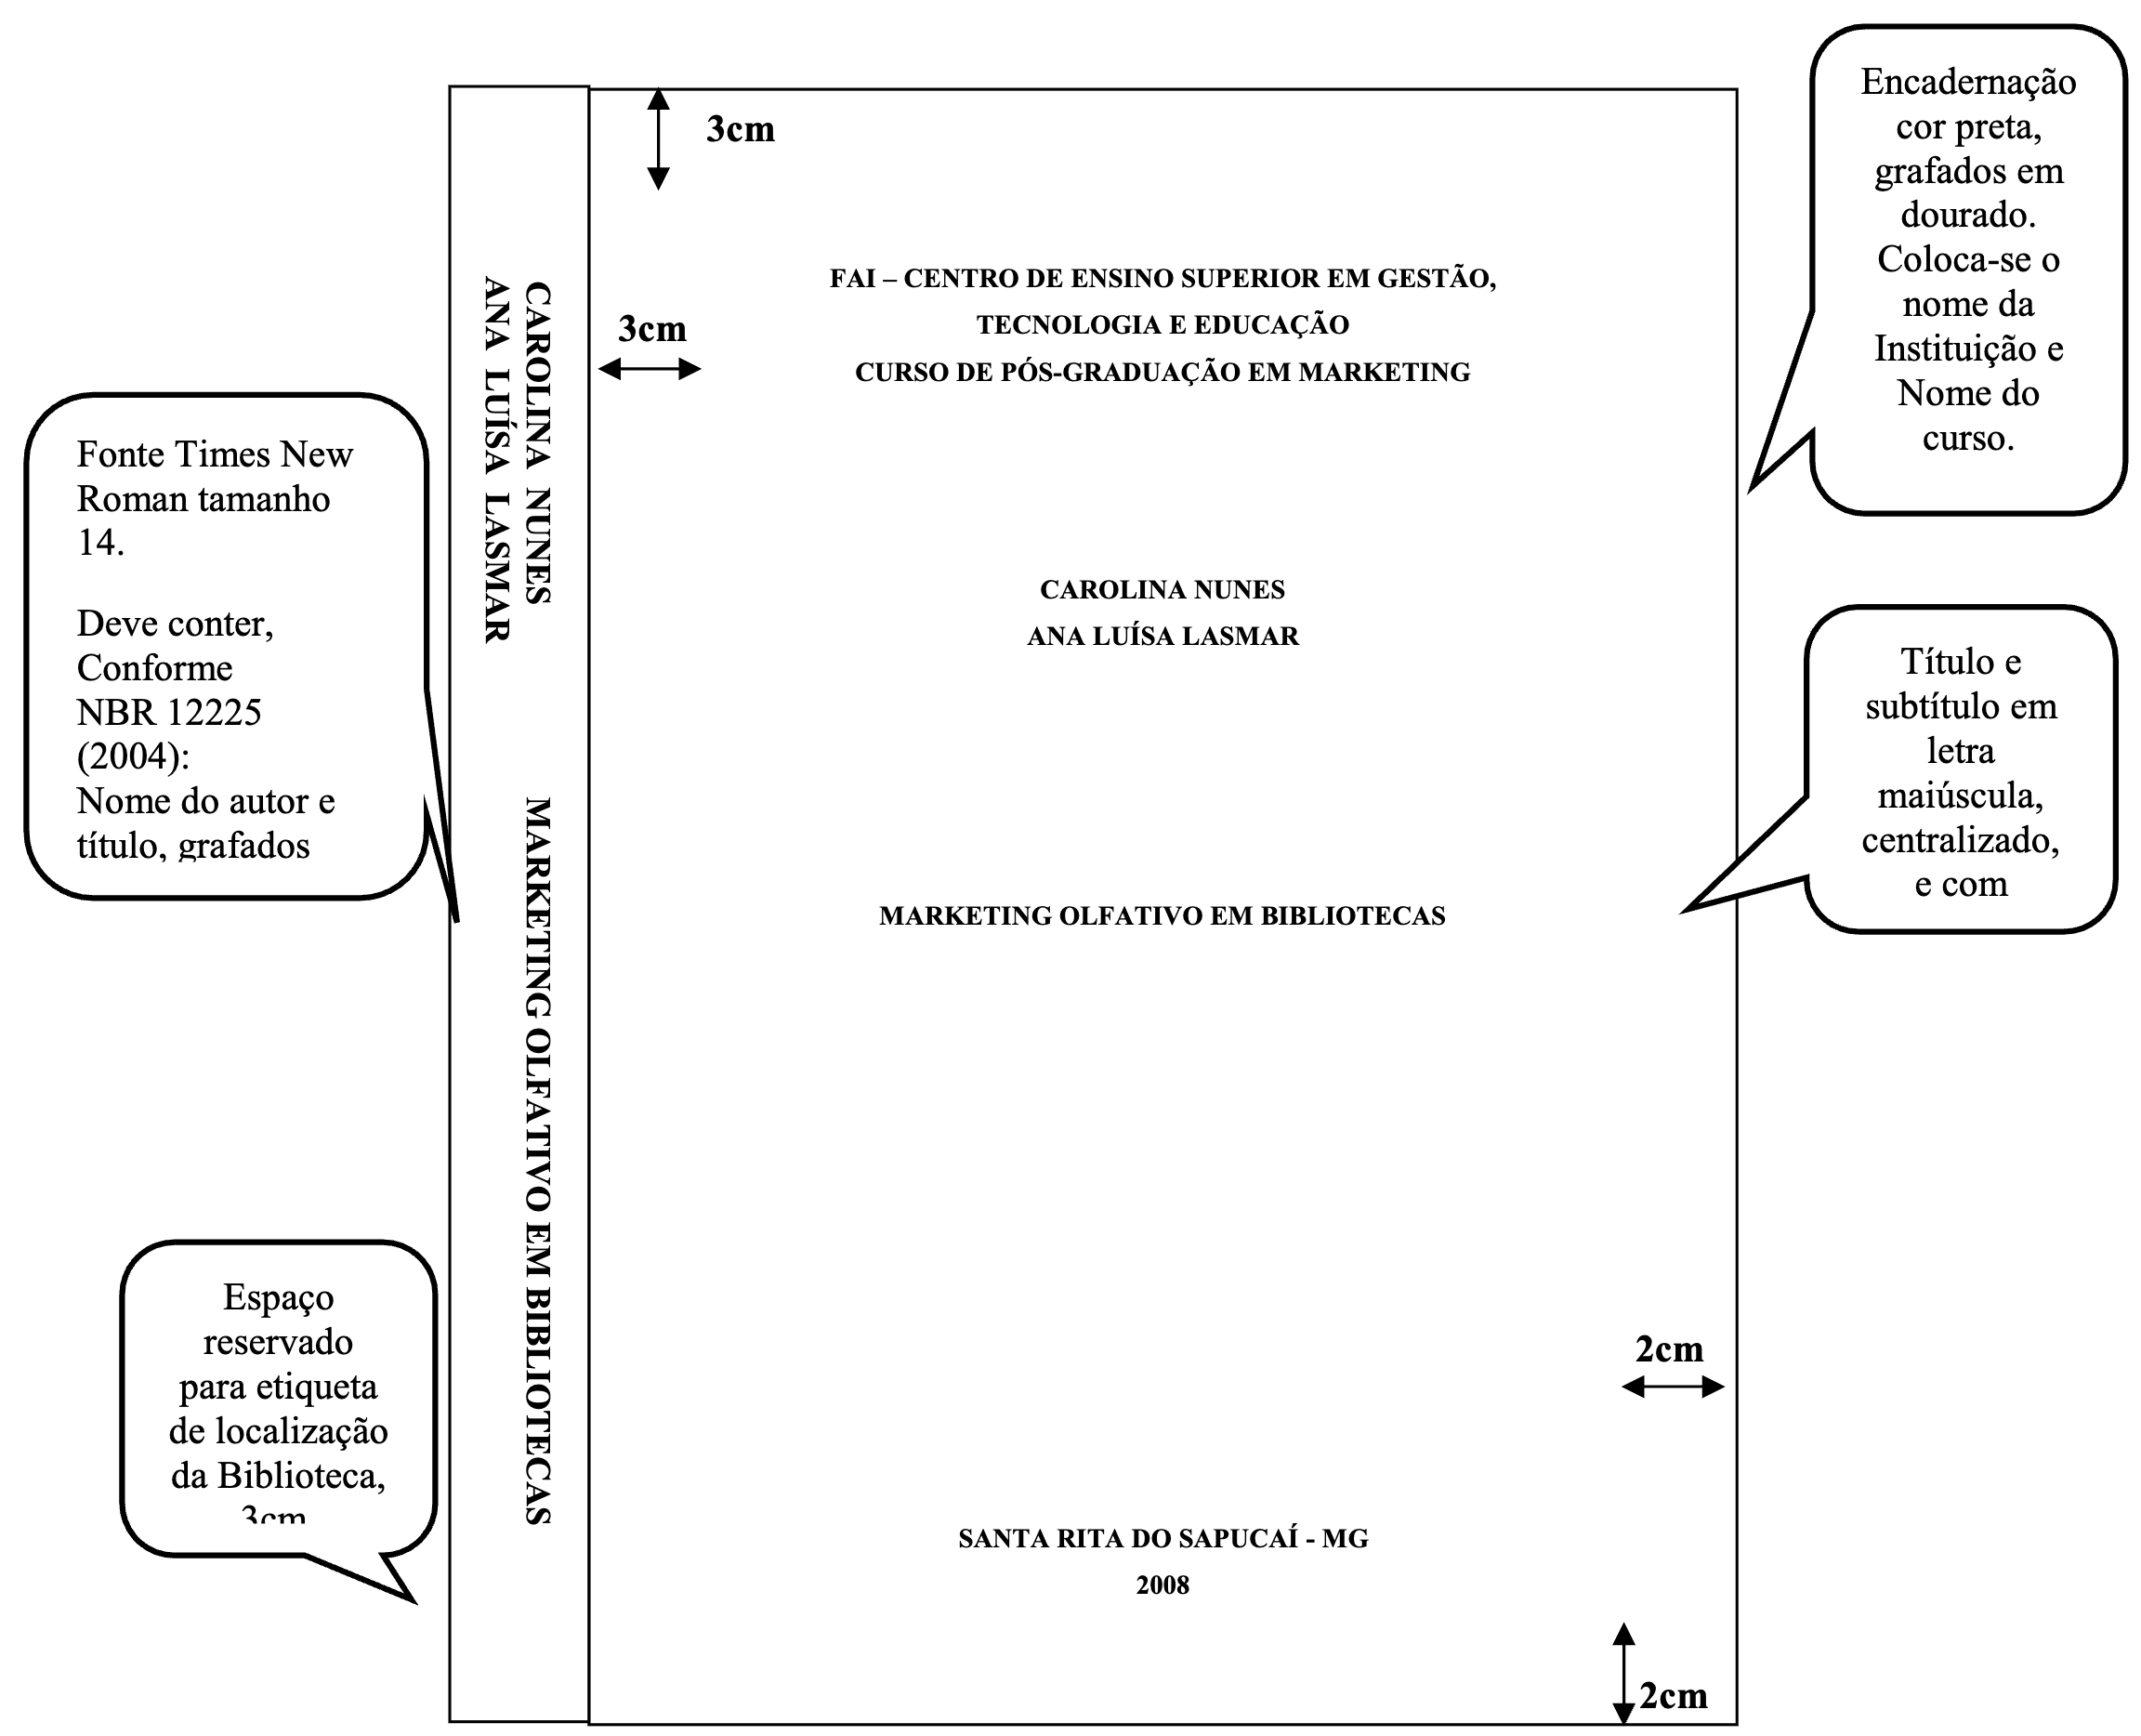
\includegraphics[width=1\textwidth]{ilustracoes/figuras/Modelo de Capa e Lombada.png}
  \legenda{Modelo de Capa e Lombada}
  \fonte{Elaboração própria}
  \label{figura:ModeloDeCapaELombada}
\end{figura}

\secaoterciaria{Capa dura e encadernação (Condicional)}
"Capa de proteção externa do trabalho sobre o qual se imprimem as informações indispensáveis à sua identificação", conforme NBR 14724 (ABNT, 2011, p. 2). A capa dura deve conter os mesmos elementos e disposição dos dados da capa ou falsa folha de rosto. Em caso de Monografia e documentação de Trabalho de Conclusão de Curso (TCC), a cópia definitiva deve ser feita com capa dura, na cor preta, com inscrições na cor dourada, para ser arquivada na Biblioteca da FAI. Os demais trabalhos devem ser encadernados com capa de plástico transparente incolor, contra capa preta e espiral também preta, ou conforme solicitação do docente.

O modelo de Capa e Lombada apresentado pela Figura 2 usa fonte de tamanho menor e serve apenas para visualização do conteúdo da folha. Os demais modelos encontram-se nos Apêndices B até Apêndice M.

A capa deve conter:
\begin{alinea}
  \item nome da Instituição;
  \item nome do curso;
  \item nome do autor;
  \item título do trabalho;
  \item subtítulo (se houver); deve ser evidenciada a sua subordinação ao título principal, precedido de dois pontos ( : );
  \item local (cidade) da instituição onde deve ser apresentado;
  \item ano de depósito (da entrega), se TCC, monografia, artigo, dissertação ou tese. Caso seja trabalho técnico-científico para avaliação bimestral ou parte deste, colocar mês/ano da entrega.
\end{alinea}

\secaosecundaria{Elementos Pré-Textuais}
Os elementos pré-textuais são apresentados pela Figura \ref{figura:ElementosPreTextuais} e nas seções seguintes.

\begin{figura}[h!]
  \centering
  \addfigura
  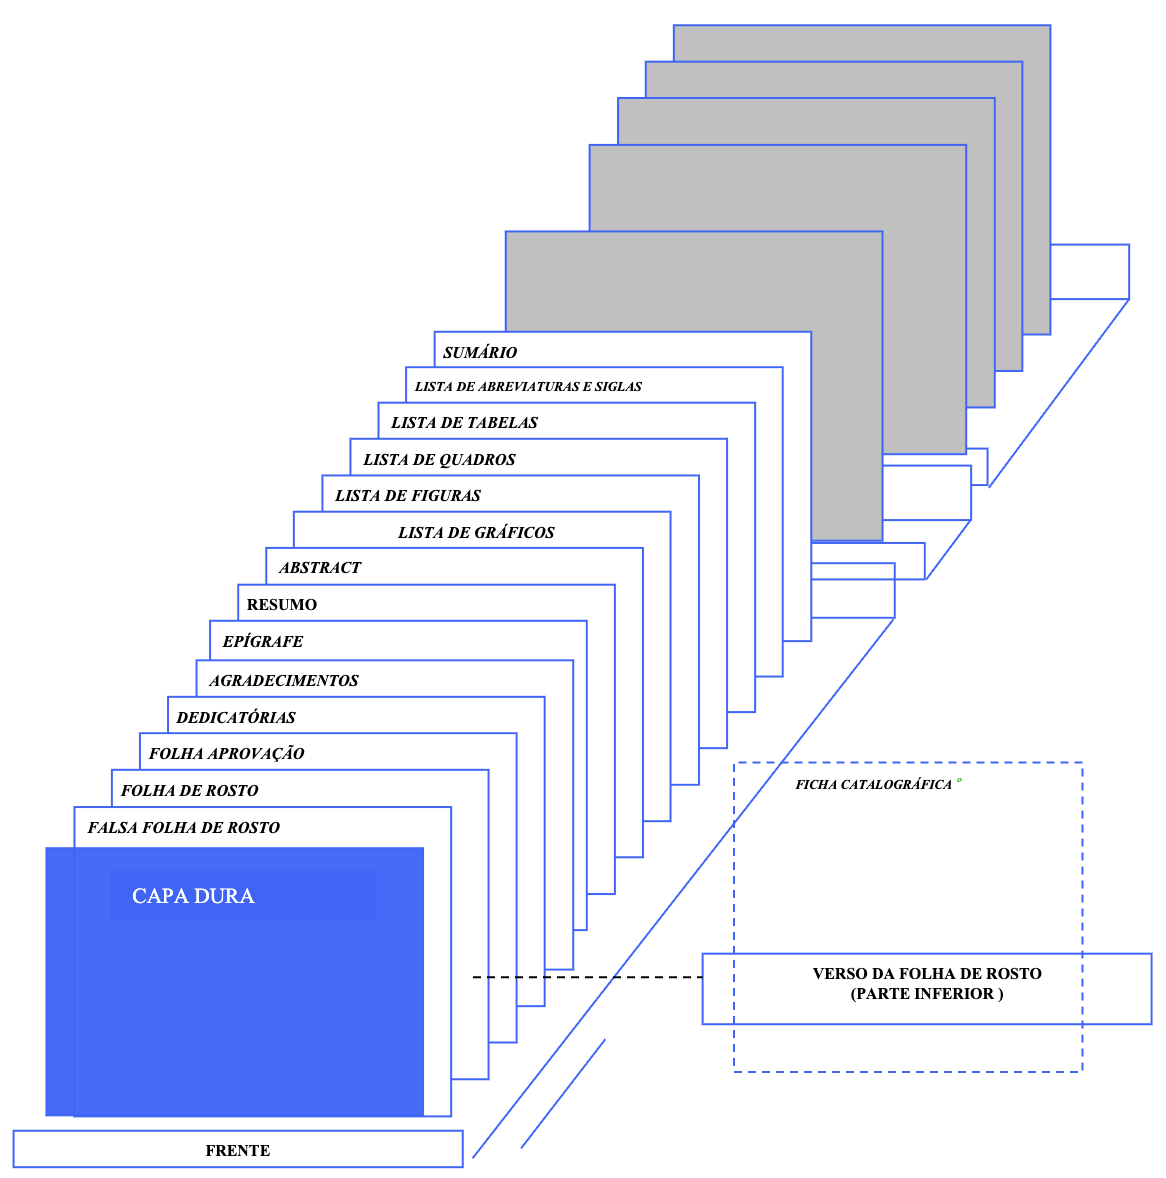
\includegraphics[width=1\textwidth]{ilustracoes/figuras/Elementos Pre Textuais.png}
  \legenda{Elementos Pré-Textuais}
  \fonte{Elaboração própria}
  \label{figura:ElementosPreTextuais}
\end{figura}

\secaoterciaria{Capa ou falsa folha de rosto (Obrigatórios)}
A capa, ou falsa folha de rosto, deve conter dados que permitam a correta identificação do trabalho: nome da Instituição, do curso, do(s) autor(es), título do trabalho e subtítulos, local e data, conforme mostra o Apêndice B.

% FIM: DESENVOLVIMENTO ================================================================
\end{Desenvolvimento}






\begin{Conclusao} % ------------------------------------------------------------------
\secaoprimaria{Conclusão}
% ============================================================================
% DESENVOLVIMENTO- EDITE O TEXTO ABAIXO. É O CONTEÚDO PRINCIPAL DO TRABALHO
% ============================================================================
...

% FIM: CONCLUSÃO==============================================================
\end{Conclusao}